% To je predloga za poročila o domačih nalogah pri predmetih, katerih
% nosilec je Tomaž Curk. Avtor predloge je Blaž Zupan.
%
% Seveda lahko tudi dodaš kakšen nov, zanimiv in uporaben element, 
% ki ga v tej predlogi (še) ni. Več o LaTeX-u izveš na
% spletu, na primer na http://tobi.oetiker.ch/lshort/lshort.pdf.
%
% To predlogo lahko spremeniš v PDF dokument s pomočjo programa
% pdflatex, ki je del standardne instalacije LaTeX programov.

\documentclass[a4paper,11pt]{article}
\usepackage{a4wide}
\usepackage{fullpage}
\usepackage[utf8x]{inputenc}
\usepackage[slovene]{babel}
\selectlanguage{slovene}
\usepackage[toc,page]{appendix}
\usepackage[pdftex]{graphicx} % za slike
\usepackage{setspace}
\usepackage{color}
\definecolor{light-gray}{gray}{0.95}
\usepackage{listings} % za vključevanje kode
\usepackage{hyperref}
\renewcommand{\baselinestretch}{1.2} % za boljšo berljivost večji razmak
\renewcommand{\appendixpagename}{Priloge}

\lstset{ % nastavitve za izpis kode, sem lahko tudi kaj dodaš/spremeniš
language=Python,
basicstyle=\footnotesize,
basicstyle=\ttfamily\footnotesize\setstretch{1},
backgroundcolor=\color{light-gray},
}

\title{Priprava podatkov in osnovne statistike podatkovne množice MovieLens}
\author{Primož Pečar (63150213)}
\date{\today}

\begin{document}

\maketitle

\section{Uvod}

V prvi domači nalogi je bil cilj, da spoznamo podatkovno množico MovieLens. Potrebno je bilo narediti analizo nad podatki o filmih. Uporabili smo osnovno znanje statistike in programiranja v Pythonu. 

\section{Podatki}

Format podatkov je bil sledeč, imeli smo csv datoteke, katere so vsebovale podatke o ocenah, žanrih, igralcih ipd. o filmih. Podatki so bili ločeni z vejicami, kjer smo imeli več podatkov za en atribut (npr. žanri), so tam bili ločeni z črto. Podatki so obsegali 9126 vrstic po excel datoteki, ker so posamezne datoteke imele drugačne atribute (cast vsebuje movID in igralce, movies vsebuje movID, ime filma, žanr etc.). Datumi so bili v posebnem formatu, katerega smo spremenili v pythonu v navaden DATE format. Ker sem uporabil znanje openpyxl, sem moral nekatere cvs datoteke convertati v xlsx.


\section{Metode}

Naloga je bila večinoma rešena v Pythonu, le za specifične grafe sem uporabil Excel, ker imam v njim že izkušnje in sem tako lahko prilagodil stil grafov. Vsaka naloga je rešena v posebaj .py datoteki. Večinoma sem uporabljal numpy, openpyxl ter zelo veliko slovarjev (defaultdict). Podatke sem prebral v arraye in jih nato obikoval v tak format, da sem lahko učinkovito reševal naloge


\section{Naloge podrobno}

V tem odseku bom opisal vsako od nalog bolj podrobno. Govoril bom o ugotovitvah, do katerih sem prišel med nalogo in zanimivostih, ki sem jih srečal.

\subsection{Naloga 1}

V nalogi 1.1 je bilo potrebno izpisati 10 najbolj ocenjenih filmov. Lotil sem se tako, da sem vse potrebne atribute naložil v posebaj array (tukaj sem tudi uporabil funkcijo datetime.fromtimestamp, za convertance int v DATE). Da sem dobil povprečje za vsak filem sem njihovo skupno vsoto ocen delil s številom ocen, v primeru da film ni bil ocenjen, sem tam zapisal nan. Podatke sem imel v obliki slovarja, kjer je bil ključ movieID, value pa float povprečja ocen. Upošteval sem samo filme, ki imajo 30 ali več ocen, ker so v podatkovni množici filmi, ki so ocenjeni enkrat in imajo oceno 5.

Stvar, ki bi jo izpostavil je sortiranje defaultdicta z lambdo, nekako sem moral dobiti 10 najbolj ocenjenih filmov, vendar sem moral sortirati slovar, kar pa ni tako enostavno. Koda je bila sledeča: 

\begin{lstlisting}
topTrueFilmi = sorted(trueAvgRatings.items(), key=lambda v: v[1], reverse=True)[:10]
\end{lstlisting}

Nato sem imel še probleme, ker numpy ni hotel prebrati movies.csv, tukaj sem uporabil openpyxl. Movies datoteko sem convertal v xlsx in nato šel čez vse celice in jih splittal. Tako sem potem povezal movieID iz movies in ratings. Končna tabela filmov je izgledala sledeče:

\begin{table}[htbp]
	\caption{Filmi in njihove povprečne ocene.}
	\label{tab_genres}
	\begin{center}
		\begin{tabular}{llp{3cm}}
			\hline
			Ime filma & Povprečen rating \\
			\hline
			Godfather            & 4.487500 \\
			Shawshank Redemption & 4.487138 \\  
			All About Eve 		 & 4.434211 \\
			African Queen        & 4.420000 \\
			Roger and Me 		 & 4.392857 \\
			Maltese Falcon       & 4.387097 \\
			Godfather: Part II   & 4.385185 \\
			Usual Suspects       & 4.370647 \\
			Modern Times 		 & 4.359375 \\
			Philadelphia Story   & 4.351351 \\
			\hline
		\end{tabular}
	\end{center}
\end{table}
\pagebreak
\subsection{Naloga 2}
V drugi nalogi je bilo potrebno poiskati kolikokrat se pojavi določen žaner, in to prikazati z ustreznim grafom. Nalaganje podatkov je praktično enako, kot v prvi. Kar je tukaj drugače je da splittamo po žanrih z delimiterjem "|" in dodajamo v slovar kjer je ključ žanr in vrednost št. pojavitev tega žanra. Ignoriramo IMAX saj v README.txt ni omenjen v skupini žanrov. Vseh žanrov je 19.


\begin{figure}[htbp]
\begin{center}
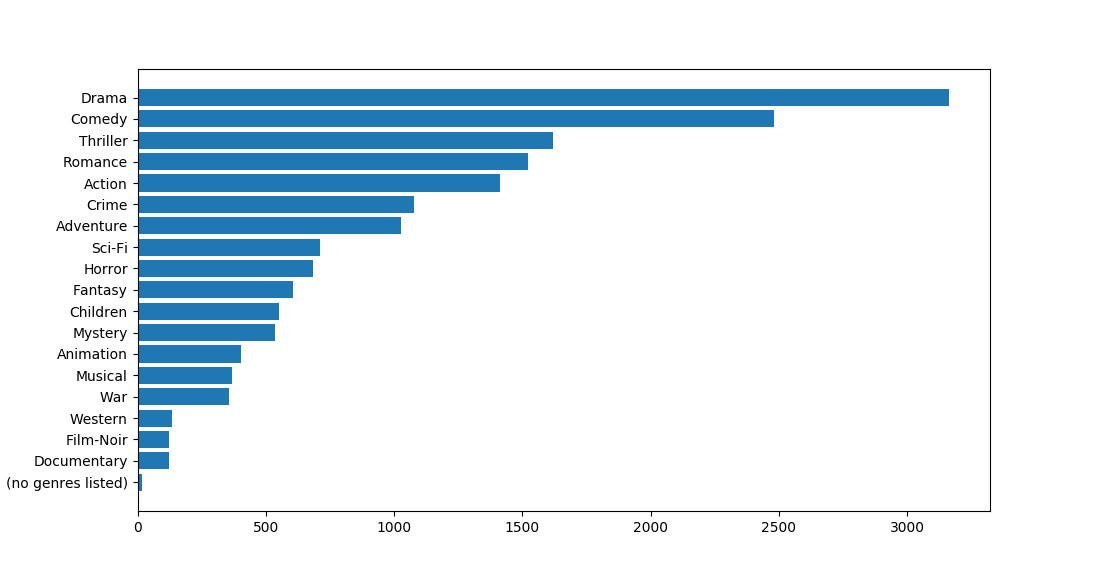
\includegraphics[scale=0.6]{../slike/zanri_porazdelitev.png}
\caption{Padajoča porazdelitev žanrov.}
\label{zanri_slika}
\end{center}
\end{figure}
\pagebreak


\subsection{Naloga 3}
V tretji nalogi je bilo potrebno pogledati, kako se spremnija povprečna ocena filma glede na njegovo gledanostjo. Ker nimamo podatke o ogledih, sem uporabil ratinge, kjer je en rating=en ogled. Izračunal sem povprečje za vsak film in jih potem razvrstil v dve kategorije, najmanj gledani in največ gledani. Obe kategorije imata 10 predstavnikov, za najmanj ogledane filme sem začel šteti šele pri 30 ogledih, saj imajo nekateri filmi le 1 ogled. Za primerjavo, najbolj ogledan filem ima 341 ogledov, najmanj ogledan pa 31. Ugotovimo da so filmi, ki imajo več ogledov imajo tudi boljšo povprečno oceno, kot tisti, ki so manj.

\begin{table}[htbp]
	\caption{Padajoče ocenjeni filmi}
	\label{tab_pad}
	\begin{center}
		\begin{tabular}{llp{3cm}}
			
			\hline
			Forrest Gump (1994) 						& 4.054252 & 341 \\
			Pulp Fiction (1994)		   					& 4.487138 & 324 \\  
			The Shawshank Redemption (1994)				& 4.487138 & 311 \\
           	Silence of the Lambs, The (1991)			& 4.138157 & 304 \\
			Star Wars: Episode IV - A New Hope (1977)	& 4.221649 & 291 \\
			\hline
		\end{tabular}
	\end{center}
\end{table}

\begin{table}[htbp]
	\caption{Naraščujoče ocenjeni filmi}
	\label{tab_nar}
	\begin{center}
		\begin{tabular}{llp{3cm}}
			\hline
			Ime filma & Povprečen rating & Število ocen \\
			\hline
			Dune (1984)			 				& 3.0833333  	& 30 \\
			National Lampoon's Vacation (1983)  & 3.6833333 	& 30 \\  
			Panic Room (2002)					& 3.2166666 	& 30 \\
			The Bone Collector (1999)			&2.88333333 	& 30 \\
			The Jungle Book (1994)				& 4.221649 		& 30 \\
			\hline
		\end{tabular}
	\end{center}
\end{table}
\pagebreak

\subsection{Naloga 4}
V četrti nalogi smo morali preveriti povezanost med timestampom ter povprečno oceno filma za tisti časovni odsek. V python kodi sem naredil primere za 4 filme, 2 najbolje ocenjena (Godfather, Shawshank Redemption) in 2 narslabše ocenjena (Home Alone,Charlie's angels). Preverjal sem kako se je za nek zelo dober filem čez čas spreminjala ocena, ter kako za nek slab film. Ugotovil sem, da ocena bolj ali manj kroži okoli splošnega povprečja filma.

\begin{figure}[htbp]
		\begin{center}
		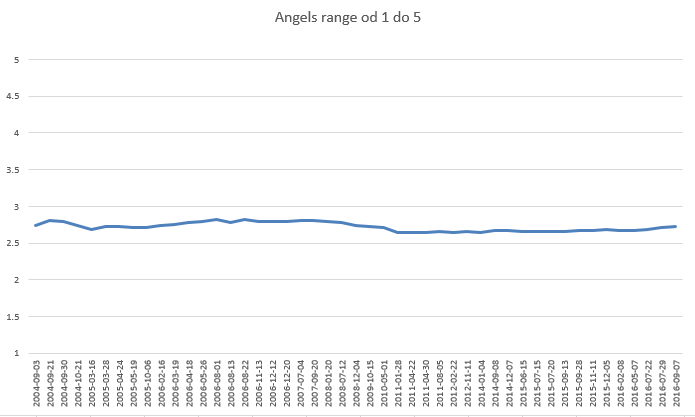
\includegraphics[scale=0.8]{../slike/agnels_range.png}
		\caption{Porazdelitev Angelov}
		\label{angeli_range}
		\end{center}
\end{figure}


\begin{figure}[htbp]
	\begin{center}
		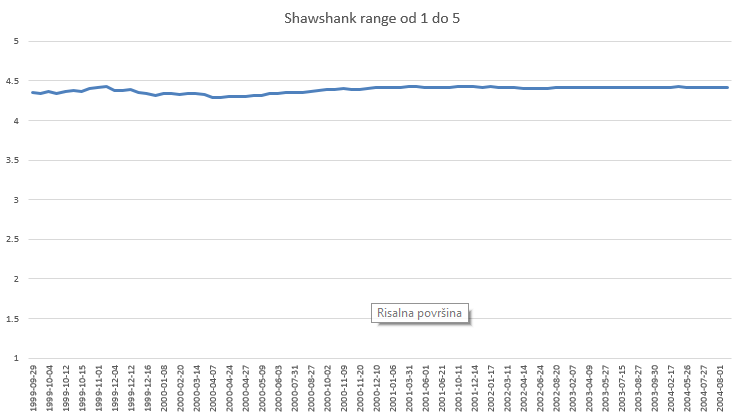
\includegraphics[scale=0.8]{../slike/shawshank_range.png}
		\caption{Porazdelitev Shawshank}
		\label{shawk_range}
	\end{center}
\end{figure}

\begin{figure}[htbp]
	\begin{center}
		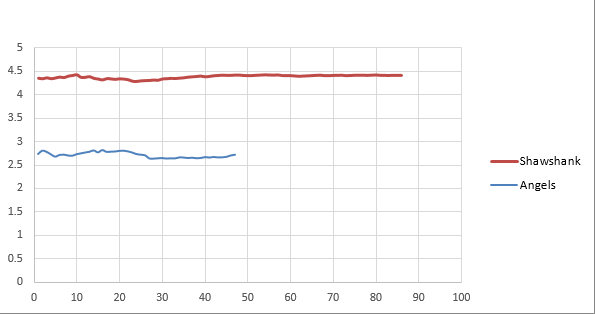
\includegraphics[scale=0.9]{../slike/skupno_ocene.png}
		\caption{Ponazorjen primer povprečnih ocen zgornjih filmov, glede na št. ocen}
		\label{skupno_range}
	\end{center}
\end{figure}
\pagebreak
 
\subsection{Naloga 5}
V peti nalogi smo morali ugotoviti, kateri so najbolj popularni igralci. Vzel sem 500 najbolj ocenjenih filmov in pogledal kateri igralci so igrali v teh filmih. To sem združil v slovar kjer je key igralec, vrednost pa št. pojavitev v igranih filmih. Potem sem vzel slovar, ga sortiral padajoče in izpisal prvih 10 igralcev, to pa sem vizualiziral v histogramu. 

\begin{figure}[htbp]
	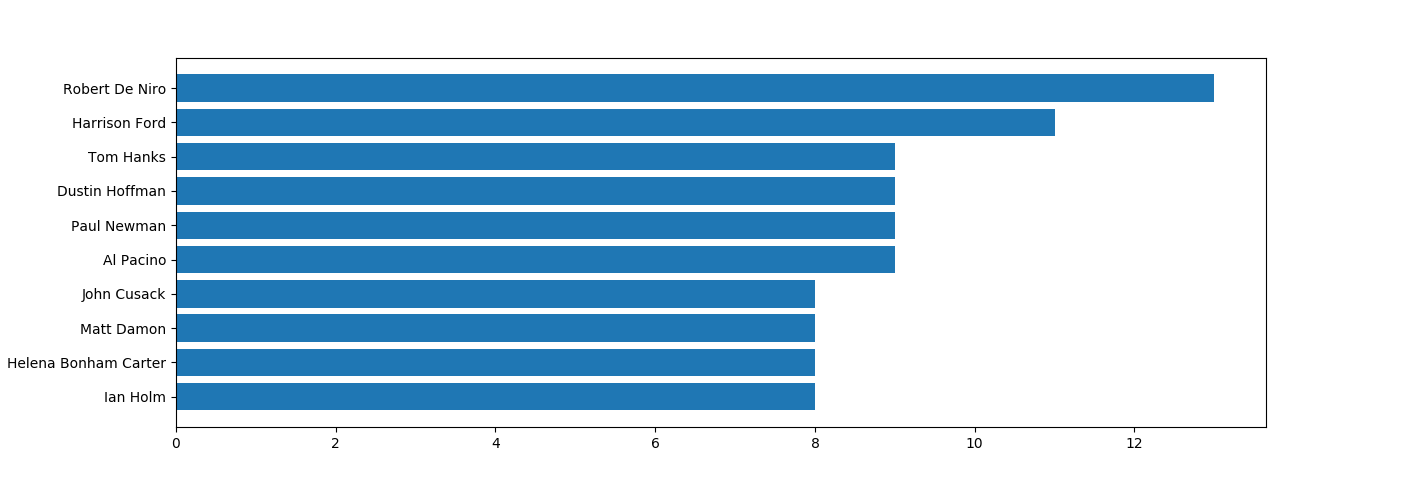
\includegraphics[scale=0.55]{../slike/pop_actors.png}
	\caption{Ponazorjen primer povprečnih ocen zgornjih filmov, glede na št. ocen}
	\label{pop_act}
\end{figure}


\subsection{Naloga 6}
The Grand Budapest Hotel, nevem kaj je s tem filmom, ampak način kako je bila zgodba prikazana, in da se film ne jemlje preveč resno mi je bil zelo všeč.
\pagebreak


\section{Rezultati}

Tukaj pa so bolj posplošeni rezultati za vsako od nalog.
  Prva naloga enačimo movieID od ratinov in moviev, združimo ratinge in imena filmov in izpišemo v padajočem vrstnem redu.
  
  Duga naloga samo splittamo žanre in povečujemo nek counter, vsakič ko se pojavi določen žanr.
  
  Tretja naloga gledamo najmanj in najbolj gledane filme in njihove povprečne ocene, ugotovimo, da so filmi bolj ali manj nagnjeni k povprečju, brez nekih hudih izjem.
  
  Četrta naloga vzamemo rating in datum ko je bil ocenjen, spremljamo kako se spreminja povprečje od začetka do "konca". Ugotovimo, da že od začetka dobro ocenjeni filmi ostanejo z dobrim povprečjem in obratno za slabe.
  
  Peta naloga pa vzamemo 500 najboljših filmov in iz actors jemljemo igralce, povečujemo counter, za vsakega izmed igralcev in na koncu izpišemo 10 najpopularnejših igralcev.
  

\section{Izjava o izdelavi domače naloge}
Domačo nalogo in pripadajoče programe sem izdelal sam.

\appendix
\appendixpage
\section{\label{app-res}Slike in programska koda}

Slike se nahajajo v mapi slike, programska koda v source, LaTex datoteke pa v tex.



\end{document}
